% ===================================================================
%  Week 8 — Thresholding & Segmentation
% ===================================================================
\documentclass[10pt,aspectratio=169]{beamer}
% ===================================================================
%  Shared Beamer preamble for "Practical Image Processing"
%  English slides. Compile with pdfLaTeX.
% ===================================================================

\usetheme{metropolis}
\usepackage[T1]{fontenc}
\usepackage[utf8]{inputenc}
\usepackage{lmodern}
\usepackage{listings}
\usepackage{tcolorbox}
\usepackage{fontawesome5}
\usepackage{booktabs}
\usepackage{amsmath,amssymb}
\usepackage{tikz}
\usepackage{pgfplots}
\pgfplotsset{compat=1.17}
\usetikzlibrary{arrows.meta,positioning,shapes.geometric,fit,backgrounds,matrix}
\tcbuselibrary{skins,breakable}

% ---- Palette --------------------------------------------------------
\definecolor{coursePrimary}{HTML}{1B4965}   % deep blue
\definecolor{courseAccent}{HTML}{E76F51}    % coral
\definecolor{courseGood}{HTML}{2A9D8F}      % teal
\definecolor{courseBad}{HTML}{C0392B}       % red
\definecolor{courseInfo}{HTML}{2980B9}      % blue
\definecolor{codeBg}{HTML}{F5F6FA}
\definecolor{codeKw}{HTML}{8E44AD}
\definecolor{codeStr}{HTML}{2A9D8F}
\definecolor{codeCom}{HTML}{7F8C8D}

\setbeamercolor{frametitle}{bg=coursePrimary}
\setbeamercolor{progress bar}{fg=courseAccent}
\setbeamercolor{alerted text}{fg=courseAccent}
\metroset{block=fill,sectionpage=progressbar,numbering=fraction}

% ---- Code listings (Python is built into listings) -----------------
\lstdefinestyle{course}{
  backgroundcolor=\color{codeBg},
  basicstyle=\ttfamily\scriptsize,
  keywordstyle=\color{codeKw}\bfseries,
  stringstyle=\color{codeStr},
  commentstyle=\color{codeCom}\itshape,
  numberstyle=\tiny\color{codeCom},
  numbers=left, numbersep=6pt,
  showstringspaces=false, breaklines=true, breakatwhitespace=true,
  tabsize=4, columns=fullflexible,
  frame=single, framesep=4pt, rulecolor=\color{gray!30},
  keepspaces=true, upquote=true, language=Python,
}
\lstset{style=course}
\lstdefinelanguage{bash}{
  keywords={cd,pip,python,venv,source,import}, sensitive=true,
  morecomment=[l]{\#}, morestring=[b]', morestring=[b]",
}

% ---- Reusable callout boxes ----------------------------------------
\newtcolorbox{goodbox}[1][Good practice]{colback=courseGood!8,colframe=courseGood,
  fonttitle=\bfseries,title={\faCheck~#1},boxrule=0.6pt,left=4pt,right=4pt,top=3pt,bottom=3pt}
\newtcolorbox{badbox}[1][Pitfall]{colback=courseBad!8,colframe=courseBad,
  fonttitle=\bfseries,title={\faTimes~#1},boxrule=0.6pt,left=4pt,right=4pt,top=3pt,bottom=3pt}
\newtcolorbox{infobox}[1][Note]{colback=courseInfo!8,colframe=courseInfo,
  fonttitle=\bfseries,title={\faInfoCircle~#1},boxrule=0.6pt,left=4pt,right=4pt,top=3pt,bottom=3pt}
\newtcolorbox{mathbox}[1][Math]{colback=coursePrimary!6,colframe=coursePrimary,
  fonttitle=\bfseries,title={\faCalculator~#1},boxrule=0.6pt,left=4pt,right=4pt,top=3pt,bottom=3pt}

\newcommand{\keyidea}[1]{\begin{alertblock}{Key idea}#1\end{alertblock}}
\newcommand{\term}[1]{\textbf{\color{coursePrimary}#1}}
\newcommand{\code}[1]{\lstinline[basicstyle=\ttfamily\small]|#1|}

% ---- A helper to draw a small pixel grid, cells shaded by value ----
% \pixelgrid{ {10,20,120,200,240}, {30,60,130,180,230}, ... }
\newcommand{\pixelgrid}[1]{%
  \begin{tikzpicture}[font=\scriptsize,scale=0.6]
    \foreach \row [count=\ry] in {#1} {
      \foreach \val [count=\cx] in \row {
        \draw[gray,fill=coursePrimary!8] (\cx,-\ry) rectangle ++(1,-1);
        \node at (\cx+0.5,-\ry-0.5) {\val};
      }
    }
  \end{tikzpicture}}


\title{Segmentation}
\subtitle{Week 8 — Splitting an image into regions}
\author{Practical Image Processing}
\date{Lecture 8 \textbullet\ 60--70 min}

\begin{document}

\maketitle

\begin{frame}{Recap \& today}
  \begin{columns}[T]
    \begin{column}{0.58\textwidth}
      \begin{itemize}
        \item Wk2/7: thresholding + morphology give clean binary shapes.
        \item \alert{Today:} \term{segmentation} — partitioning an image into meaningful regions
              (object vs background, or each object separately).
      \end{itemize}
    \end{column}
    \begin{column}{0.42\textwidth}
      \begin{alertblock}{DocScan milestone}
        Segment each digit as its own region, even when two digits touch — so they can be read
        one at a time.
      \end{alertblock}
    \end{column}
  \end{columns}
\end{frame}

\begin{frame}{Roadmap}\tableofcontents\end{frame}

% ==================================================================
\section{Threshold-based segmentation}
% ==================================================================

\begin{frame}{Segmentation = assign each pixel a label}
  \begin{itemize}
    \item The goal: group pixels into regions that mean something (a digit, the page, the sky).
    \item Simplest case: two labels (object / background) $=$ \term{thresholding} (Week 2).
    \item Harder: many objects, touching objects, or regions defined by color/texture.
  \end{itemize}
  \keyidea{Segmentation is where ``pixels'' become ``objects.'' Everything downstream (counting, reading) depends on it.}
\end{frame}

\begin{frame}{Global vs adaptive threshold — on the meter}
  \begin{columns}[T]
    \begin{column}{0.33\textwidth}\begin{center}
      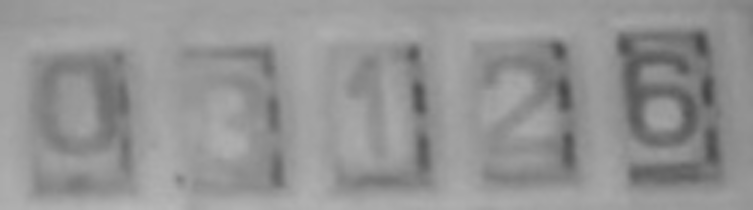
\includegraphics[width=\linewidth]{../assets/gray.png}\\{\scriptsize gray}
    \end{center}\end{column}
    \begin{column}{0.33\textwidth}\begin{center}
      
\includegraphics[width=\linewidth]{../assets/otsu.png}\\{\scriptsize global Otsu}
    \end{center}\end{column}
    \begin{column}{0.33\textwidth}\begin{center}
      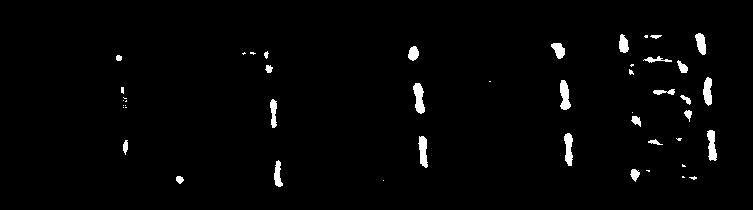
\includegraphics[width=\linewidth]{../assets/adaptive.png}\\{\scriptsize adaptive}
    \end{center}\end{column}
  \end{columns}
  \vspace{3pt}
  Otsu picks one global threshold (great for even lighting); adaptive computes a local one
  (robust to shadows). Recall Week 2 — this is our starting point.
\end{frame}

\begin{frame}{Otsu, revisited}
  \begin{itemize}
    \item Finds the threshold that best separates the two histogram modes (max between-class variance).
    \item Works when the histogram is clearly \term{bimodal} (object vs background).
    \item Fails on: uneven lighting, more than two classes, or a unimodal histogram.
  \end{itemize}
  \begin{mathbox}
    Maximize $\sigma_B^2(t)=w_0(t)\,w_1(t)\,[\mu_0(t)-\mu_1(t)]^2$ over the threshold $t$.
  \end{mathbox}
\end{frame}

% ==================================================================
\section{Region-based segmentation}
% ==================================================================

\begin{frame}{Beyond thresholds}
  \begin{itemize}
    \item \term{Region growing}: start from seeds, add neighbours that are similar enough.
    \item \term{Split-and-merge}: divide the image, then merge regions that are alike.
    \item \term{Color/k-means}: cluster pixels by color into $k$ regions.
  \end{itemize}
  \keyidea{Thresholding uses only intensity; region methods use \emph{similarity and connectivity} — more powerful, more parameters.}
\end{frame}

\begin{frame}{k-means colour segmentation — real car}
  \begin{columns}[T]
    \begin{column}{0.5\textwidth}\begin{center}
      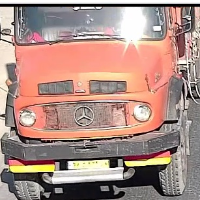
\includegraphics[width=0.85\linewidth]{../assets/car.png}\\{\scriptsize original}
    \end{center}\end{column}
    \begin{column}{0.5\textwidth}\begin{center}
      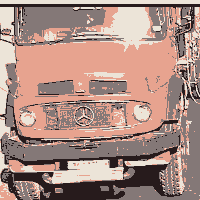
\includegraphics[width=0.85\linewidth]{../assets/car_kmeans.png}\\{\scriptsize k-means, $k$=4 colours}
    \end{center}\end{column}
  \end{columns}
  \vspace{3pt}
  \begin{itemize}
    \item Each pixel is a point in (R,G,B); k-means groups them into $k$ clusters.
    \item Replace each pixel by its cluster's colour $\rightarrow$ a segmented, posterized image.
  \end{itemize}
\end{frame}

\begin{frame}{k-means: how it works}
  \begin{enumerate}
    \item Pick $k$ initial cluster centres.
    \item Assign each pixel to the nearest centre.
    \item Recompute each centre as the mean of its pixels.
    \item Repeat 2--3 until stable.
  \end{enumerate}
  \begin{badbox}
    You must choose $k$; the wrong $k$ over- or under-segments. It also ignores \emph{position} — only colour.
  \end{badbox}
\end{frame}

% ==================================================================
\section{Watershed: separating touching objects}
% ==================================================================

\begin{frame}{The touching-objects problem}
  \begin{itemize}
    \item Threshold + morphology gives blobs — but two touching digits become \emph{one} blob.
    \item Counting/reading needs them separated. Erosion helps a little, but can break thin strokes.
    \item \term{Watershed} solves it properly, using the shape (a distance transform).
  \end{itemize}
\end{frame}

\begin{frame}{Distance transform $\rightarrow$ watershed}
  \begin{columns}[T]
    \begin{column}{0.5\textwidth}\begin{center}
      
\includegraphics[width=0.9\linewidth]{../assets/distance.png}\\{\scriptsize distance transform}
    \end{center}\end{column}
    \begin{column}{0.5\textwidth}\begin{center}
      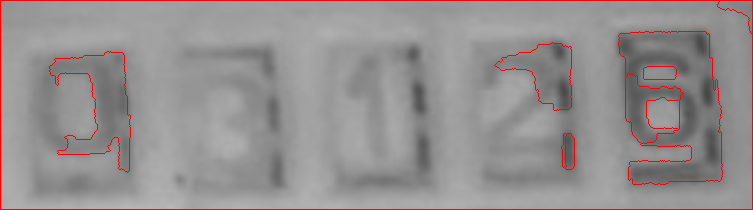
\includegraphics[width=0.9\linewidth]{../assets/watershed.png}\\{\scriptsize watershed boundaries (red)}
    \end{center}\end{column}
  \end{columns}
  \vspace{3pt}
  The distance transform peaks at each object's centre; watershed ``floods'' from those peaks and
  builds a ridge where floods meet — the separating boundary.
\end{frame}

\begin{frame}{Watershed intuition}
  \begin{itemize}
    \item Treat intensity (or $-$distance) as a landscape; ``water'' rises from marked minima.
    \item Where two catchment basins meet, build a dam — that dam is the object boundary.
    \item \term{Markers} (seeds) control it, or it \term{over-segments} (every tiny minimum a region).
  \end{itemize}
  \begin{goodbox}
    Marker-controlled watershed is the reliable version: you tell it the sure-foreground and sure-background.
  \end{goodbox}
\end{frame}

\begin{frame}[fragile]{Watershed in code (marker-controlled)}
\begin{lstlisting}[language=Python]
dist = cv2.distanceTransform(binary, cv2.DIST_L2, 5)
_, sure_fg = cv2.threshold(dist, 0.5*dist.max(), 255, 0)  # digit centres
sure_bg = cv2.dilate(binary, k, iterations=3)
unknown = cv2.subtract(sure_bg, np.uint8(sure_fg))
_, markers = cv2.connectedComponents(np.uint8(sure_fg))
markers = markers + 1; markers[unknown==255] = 0
markers = cv2.watershed(color_img, markers)               # -1 = boundaries
\end{lstlisting}
\end{frame}

% ==================================================================
\section{Connected components}
% ==================================================================

\begin{frame}{Labelling separate blobs}
  \begin{columns}[T]
    \begin{column}{0.55\textwidth}\begin{center}
      
\includegraphics[width=0.95\linewidth]{../assets/components.png}\\{\scriptsize each blob a different colour}
    \end{center}\end{column}
    \begin{column}{0.45\textwidth}
      \begin{itemize}
        \item \term{Connected components} labels each separate white region with an integer.
        \item Once separated, each digit is its own component you can crop and read (Week 9).
        \item \code{cv2.connectedComponents} / \code{...WithStats} give labels + areas + boxes.
      \end{itemize}
    \end{column}
  \end{columns}
\end{frame}

% ==================================================================
\section{In-class exercise}
% ==================================================================

\begin{frame}{\faPen~In-class exercise (12 min)}
  \begin{infobox}[Choose a method]
  \end{infobox}
  Which segmentation method fits each task?
  \begin{enumerate}
    \item Separate dark text from a light page under even lighting.
    \item Two meter digits are touching and must be counted separately.
    \item Segment a photo into ``sky / road / car'' regions by colour.
    \item A document photographed with a shadow across half of it.
  \end{enumerate}
\end{frame}

\begin{frame}{\faPen~Debrief}
  \begin{itemize}
    \item (1) Even lighting, bimodal $\rightarrow$ \term{Otsu}. (2) Touching objects $\rightarrow$ \term{watershed}.
    \item (3) Colour regions $\rightarrow$ \term{k-means} (or colour thresholding in HSV).
    \item (4) Shadow $\rightarrow$ \term{adaptive} threshold (local), not global Otsu.
  \end{itemize}
  \keyidea{No single method wins. Match the method to the structure: intensity, colour, connectivity, or lighting.}
\end{frame}

% ==================================================================
\section{Deep dive}
% ==================================================================

\begin{frame}{Evaluating a segmentation}
  \begin{itemize}
    \item With ground-truth masks: \term{IoU} (intersection over union) and \term{Dice} score.
    \item Over-segmentation (too many regions) vs under-segmentation (merged regions) — both are errors.
    \item For DocScan: the real test is downstream — can each digit be read after segmentation?
  \end{itemize}
  \begin{mathbox}
    $\mathrm{IoU}=\dfrac{|A\cap B|}{|A\cup B|}$ — 1.0 is perfect overlap with the truth.
  \end{mathbox}
\end{frame}

\begin{frame}{Classical vs deep segmentation}
  \begin{itemize}
    \item Classical (threshold/watershed/k-means): fast, interpretable, no training — great for clean, structured images.
    \item Deep (U-Net, Mask R-CNN, SAM): learns to segment complex scenes, but needs data/compute.
    \item For meters/documents, classical often suffices; deep shines on messy natural scenes (Week 13--14).
  \end{itemize}
\end{frame}

\begin{frame}{GrabCut \& graph-based methods (brief)}
  \begin{itemize}
    \item \term{GrabCut}: model foreground/background colour distributions and cut the graph optimally — interactive object cutout.
    \item Graph-cut/normalized-cut view segmentation as partitioning a pixel graph.
    \item These bridge classical and modern; good to know they exist.
  \end{itemize}
\end{frame}

\begin{frame}{The segmentation pipeline for DocScan}
  \begin{center}
  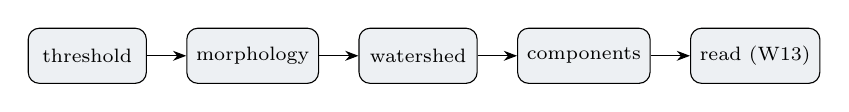
\begin{tikzpicture}[font=\scriptsize,>=Stealth,node distance=2mm and 5mm,
    b/.style={draw,rounded corners,fill=coursePrimary!8,minimum height=7mm,minimum width=15mm,align=center}]
    \node[b] (thr){threshold};
    \node[b,right=of thr] (mo){morphology};
    \node[b,right=of mo] (ws){watershed};
    \node[b,right=of ws] (cc){components};
    \node[b,right=of cc] (rd){read (W13)};
    \draw[->](thr)--(mo);\draw[->](mo)--(ws);\draw[->](ws)--(cc);\draw[->](cc)--(rd);
  \end{tikzpicture}
  \end{center}
  \begin{itemize}
    \item Threshold $\rightarrow$ clean $\rightarrow$ separate touching digits $\rightarrow$ label each $\rightarrow$ read.
    \item Each digit becomes an isolated image the CNN can classify.
  \end{itemize}
\end{frame}

% ==================================================================
\section{Wrap-up}
% ==================================================================

\begin{frame}{What you should now be able to do}
  \begin{itemize}
    \item Segment by threshold (global/adaptive/Otsu) and know when each fails.
    \item Use k-means for colour segmentation; region methods for similarity.
    \item Separate touching objects with a marker-controlled watershed.
    \item Label blobs with connected components; evaluate with IoU/Dice.
  \end{itemize}
\end{frame}

\begin{frame}{This week's deliverable}
  \begin{alertblock}{Due before Week 9 (see \code{project/})}
    \begin{enumerate}
      \item Compare Otsu vs adaptive on meter images; pick the winner per lighting.
      \item k-means colour segmentation of a car/plate photo at $k=2,4,8$; discuss.
      \item Watershed to separate touching meter digits; label each with connected components.
      \item DocScan milestone: output one cropped image per digit, in order.
    \end{enumerate}
  \end{alertblock}
\end{frame}

\begin{frame}[standout]
  Segmentation turns pixels into objects.\\[4pt]
  \normalsize Threshold for two classes, k-means for colour, watershed for touching objects.
\end{frame}

\end{document}
